\documentclass[12pt,a4paper]{article}
\title{%
  Øving 6 \\
  \large IFYKJT1001 - Fysikk/Kjemi \\
  }
\author{Gunnar Myhre, BIELEKTRO}

\usepackage[utf8]{inputenc}
\usepackage[norsk]{babel}
\usepackage{amsmath}
\usepackage{siunitx}

\usepackage{graphicx}
\graphicspath{ {./images} }

\setlength\parindent{0pt}

\begin{document}
  \maketitle

  \section*{Oppgåve 1}
    \begin{center}
      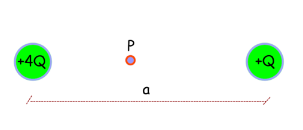
\includegraphics[scale=0.6]{06_1.png}
    \end{center}
    Vi ser etter eit punkt $P$ der feltvektorane frå kjeldeladningane $q_1 = 4Q$ og $q_2 = 1Q$
    er like, og differansen mellom dei dermed er null
    \begin{equation}
      E_{P} = E_1 - E_2 = 0 \rightarrow E_1 = E_2
    \end{equation}
    fyller inn for ladningane med Coulombs lov
    \begin{equation}
      k\frac{q_1}{b^2}\hat{\vec{r}} = 
      k\frac{q_2}{(a-b)^2}\hat{\vec{r}} \rightarrow
      \frac{4}{b^2} = \frac{1}{(a-b)^2}
    \end{equation}
    der $b$ er lengda frå $q_1 = 4Q$ til punktet $P$. Løyser algebraisk for $b$
    \begin{equation}
      4a^2 - 8ab + 3b^2 = 0 \rightarrow b=\frac{8a\pm \sqrt{64a^2 - 48a^2}}{6}
      \rightarrow b=\frac{2a}{3} \vee b = 2a
    \end{equation}
    Den første løysninga $b= \frac{2a}{3}$ ligger mellom ladningene og er derfor
    det gyldige svaret.


  \section*{Oppgåve 2}
    \begin{center}
      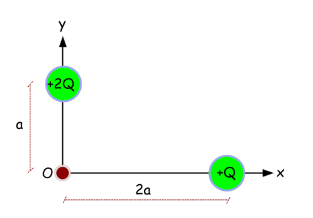
\includegraphics[scale=0.6]{06_2.png}
    \end{center}
    Det totale elektriske feltet i punktet $O$ er gitt som
    \begin{equation}
      E_{tot} = E_1 + E_2 = k\left[ \frac{q_1}{a^2} + \frac{q_2}{4^2} \right] \hat{\vec{r}}
    \end{equation}
    sidan kreftene står normalt på kvarandre kan vi bruke pytagoras for å finne størrelsen
    til $E_{tot}$
    \begin{equation}
      |E_{tot}| = \sqrt{\frac{k^2}{a^4}\left( 4Q^2 + \frac{Q^2}{4} \right) }\hat{\vec{r}}
      \rightarrow \frac{k}{a^2}\sqrt{\frac{65}{4}}Q \hat{\vec{r}}
    \end{equation}
    vinkelen mellom feltvektorane kan vi finne om vi setter inn vilkårlege verdiar for $Q$ og $a$
    \begin{equation}
      \alpha = artan\left( \frac{2Q/a^2}{Q/4a^2} \right)
      = artan\left( \frac{2}{0.25} \right) = \ang{82,9}
    \end{equation}

  \newpage

  \section*{Oppgåve 3}
    \begin{center}
      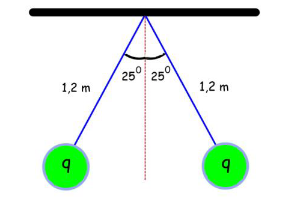
\includegraphics[scale=0.6]{06_3.png}
    \end{center}
    \subsection*{a)}
    Sidan gravitasjonskrafta $mg$ og den elektrostatiske krafta $E$ står vinkelrett
    på kvarandre stemmer dette forholdet
    \begin{equation}
      \frac{E}{mg} = tan(25)
    \end{equation}
    vi kan uttrykke $E$ vha. Coulombs lov
    \begin{equation}
      E = k\frac{q^2}{(2r)^2}
    \end{equation}
    der $r$ er distansen til vertikalen frå snorfestet. Vi kjenner nå alle mengdene og kan
    finne $q$
    \begin{equation}
      q = \sqrt{\frac{4r^2mgtan25}{k}} = 2,80\cdot10^{-6} [C]
    \end{equation}

    \subsection*{b)}
    I dette tilfellet stemmer fortsatt
    \begin{equation}
      \frac{E}{mg} = tan(\beta)
    \end{equation}
    for den nye vinkelen $\beta$, og den nye radiusen $r$ som inngår i Coulombs lov for $E$.
    Vi kan sette kjente uttrykk 
    \begin{equation}
      \frac{kq^2}{(2r)^2 mg} = tan(\beta) \longrightarrow 
      sin^2(\beta)tan(\beta) = \frac{kq^2}{1,2^2mg}
    \end{equation}
    her er det kun $\beta$ som er ukjent, og sidan det ikkje er matematiske
    metodar som er fokus her setter eg inn for kjente mengder og bruker ein
    grafisk løysar for å finne $\beta = \ang{39,5}$.


  \section*{Oppgåve 4}
    \begin{center}
      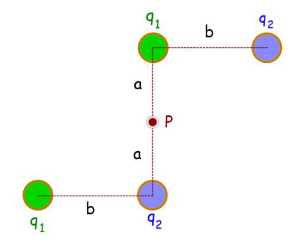
\includegraphics[scale=0.6]{06_4.png}
    \end{center}
    Vi kjenner til at det elektriske potensialet i eit punkt med avstand $r$ frå ein 
    ladning $q$ er gitt som
    \begin{equation}
      V(r) = \frac{U(r)}{q_0} \rightarrow V(r) = k\frac{q\cdot q_0}{q_0}\frac{1}{r}
      \rightarrow V = k\frac{q}{r}
    \end{equation}
    vi kan summere opp dei elektriske potensiala frå dei fire ladningene. Finner avstanden
    til dei ytterste ladningene
    \begin{equation}
      c = \sqrt{a^2 + b^2} = 0,5[m]
    \end{equation}
    finner det elektriske potensialet i punktet $P$
    \begin{equation}
      V_{P} = \sum_{i=1}^4 k\frac{q_i}{r_i} =
      \left[\frac{q_1 + q_2}{a} + 
            \frac{q_1 + q_2}{c} \right] k =
            -2,39 \cdot 10^5 [V]
    \end{equation}

  \section*{Oppgåve 5}
    \begin{center}
      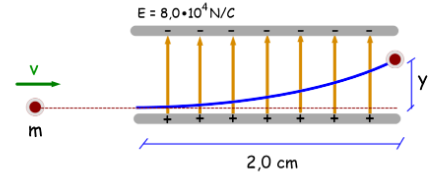
\includegraphics[scale=0.6]{06_5.png}
    \end{center}
    Ein måte å finne ladninga på er å finne akselerasjonen i y-retning.
    Finner først tida det tar for partikkelen å bevege seg $2 \si{\centi\meter}$
    \begin{equation}
      s_x = v_x t \rightarrow t= \frac{s}{v_x} \rightarrow t = \frac{2\cdot
      10^{-2}}{20} = 10^{-3}[s]
    \end{equation}
    finner farta i y-retning når partikkelen treffer veggen på andre sida
    \begin{equation}
      s_y= \frac{v_y + v_{y_0}}{2} t \rightarrow v_y = 2\frac{s_y}{t} \rightarrow
      v_y= 2\frac{3\cdot 10^{-4}}{10^{-3}} = 0,6 [m/s]
    \end{equation}
    finner akselerasjonen i y-retning
    \begin{equation}
      v_y = v_{y_0} + a_y t \rightarrow a_y = \frac{v_y}{t} \rightarrow
      a_y = \frac{0,6}{10^{-3}} = 600[m/s^2]
    \end{equation}
    vi kjenner at 
    \begin{equation}
      E = \frac{F}{q}
    \end{equation}
    setter inn for Newtons andre lov og finner $q$
    \begin{equation}
      E = \frac{ma}{q} \rightarrow q = \frac{ma}{E} = 
      \frac{1,4\cdot 10^{-8}\cdot 600}{8\cdot 10^4} = 1,05\cdot 10^{-10}[C]
    \end{equation}
    
  \section*{Oppgåve 6}
    \begin{center}
      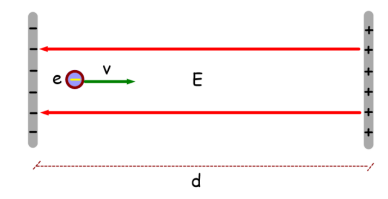
\includegraphics[scale=0.6]{06_6.png}
    \end{center}
    Setter opp likning for energibevaring
    \begin{equation}
      U_1 = K_2 + U_2 \rightarrow K_2 = U_1 - U_2 \rightarrow K_2 = q_e(V_1 - V_2)
    \end{equation}
    setter inn uttrykk for translasjon
    \begin{equation}
      \frac{1}{2}m_e v_2^2 = q_e\Delta V
    \end{equation}
    finner verdiar for elektron
    \begin{itemize}
      \item $q_e = -1,6 \cdot 10^{-19}[C]$
      \item $m_e = 9,109 \cdot 10^{-31} [kg]$
    \end{itemize}
    setter inn for kjente mengder og finner $\Delta V$
    \begin{equation}
      \Delta V = \frac{m_ev_2^2}{2q_e} = \frac{9,1\cdot 10^{-31} \cdot (3 \cdot 10^7)^2}
      {2\cdot 1,6\cdot 10^{-19}} = 2559,3[V]
    \end{equation}
    sidan vi har fått oppgitt at det elektriske feltet kan operere i størrelsesorden
    $E = 10^8 [V/m]$ kan vi finne distansen
    \begin{equation}
      d = \frac{2559,3 [V]}{10^8[V/m]} = 2,5\cdot 10^{-5}
    \end{equation}

\end{document}
